\documentclass[11pt]{article}
\usepackage[utf8]{inputenc}
\usepackage[margin=2.5cm]{geometry}
\usepackage{amsmath,amsthm,amsfonts,amssymb}
\usepackage{graphicx,latexsym}
\usepackage{float}
\usepackage{booktabs}
\usepackage{multirow}
\usepackage{cite}
\usepackage{url}
\usepackage{algorithm}
\usepackage{algpseudocode}
\usepackage{caption}
\usepackage{tikz}
\usetikzlibrary{arrows.meta,positioning,fit,backgrounds}
\renewcommand{\baselinestretch}{1.2 }

\title{\textbf{Reject-Before-Propagate: Hard-Gated Citation Checks for Automated Literature Synthesis}}

\author{\begin{tabular}{rcl}
\textbf{Harish Vidyarth N$^{\text a,}$\thanks{Corresponding author: harishvidyarth.n.2024.csecs@rajalakshmi.edu.in}, A.L. Reshma$^{\text a}$, R. Divya$^{\text a}$}
\end{tabular}\\
\\
\begin{tabular}{c}
$^{\text a}$\small Department of Computer Science and Engineering (Cyber Security), \\Rajalakshmi Engineering College, Thandalam, Chennai 602105, India \\
\end{tabular}}

\date{}

\begin{document}
\maketitle
\vspace{-0.5cm}
\begin{abstract}
{\small Large language model (LLM) pipelines are increasingly used for automated literature review, supporting tasks such as claim extraction, contradiction detection, and evidence synthesis. Existing systems, however, typically treat citation grounding as a \emph{scored} property: generated statements are checked, rated, or flagged for human review, but are not structurally prevented from reaching the final output when unsupported. We present \textbf{Verify-or-Reject Grounding (VoRG)}, an architectural pattern that treats citation grounding as a \emph{build-time invariant}. Under this approach, each stage of the literature-synthesis pipeline either produces output that can be mechanically verified against source evidence, or rejects the output before it can propagate downstream. Our reference implementation combines verbatim-substring-verified evidence extraction, deterministic synthesis-matrix aggregation, and a narrative verifier that rejects generated sentences whose citations cannot be resolved to verified evidence. The same principle is applied to contradiction detection and journal-metadata reconciliation. The full pipeline more than doubles claim-extraction F1 relative to the naive baseline (0.442 $\pm$ 0.070 vs. 0.158 $\pm$ 0.007, mean $\pm$ SD over three runs), though at this sample size a rule-based pattern-mode ablation is nominally comparable (0.510 $\pm$ 0.152), indicating the measured gain comes chiefly from decomposing extraction into per-claim stages rather than from the LLM call itself. By contrast, research-gap detection, the only major stage not yet protected by the verify-or-reject mechanism, shows low recall and produces a confirmed false positive contradicted by the reviewed corpus. This result underscores the need to extend the same verification discipline to other stages of agentic scientific NLP pipelines.}
\end{abstract}
\textbf{Keywords:} {\small Verify-or-Reject Grounding; literature synthesis; large language models; citation grounding; hallucination mitigation; scientific NLP}

\section{Introduction}

Large language models are increasingly used to accelerate literature review by extracting claims from papers, identifying disagreements between studies, and drafting synthesis narratives. A well-documented failure mode of this automation is \emph{hallucination}, in which a generated statement appears well supported but does not correspond to any statement in the source~\cite{zhang2025hallucination,ji2023survey,tonmoy2024comprehensive}. A closely related failure is citation-level: even when the surrounding text is accurate, the cited source may not actually say what the model claims, or may not exist at all~\cite{zhang2025citation}. Existing mitigation approaches commonly rely on post-hoc verification, in which a claim or generated passage is checked against retrieved evidence and assigned a score, flagged, or routed for human review~\cite{li2025enhancing}. Because validation in this scheme is a signal appended to the output rather than a gatekeeper that controls it, an unverified or contradictory statement can still reach the user if the score is not acted on.

This paper presents an alternative design principle, \textbf{Verify-or-Reject Grounding (VoRG)}. The distinction matters because synthesis output from pipelines like this one is often consumed downstream by people making real decisions, such as a systematic-review team drafting a submission~\cite{li2025enhancing}; a hallucinated citation that merely lowers a confidence score, rather than being blocked outright, carries a correspondingly higher cost in that setting. Section~\ref{sec:method} formalizes VoRG's rejection semantics. The evaluation is deliberately narrow, using a single gold-annotated topic and three repeated runs, but is based entirely on reproducible pipeline output rather than illustrative or hypothetical results.

Our contributions are:
\begin{enumerate}
 \item A formal description of Verify-or-Reject Grounding as a reusable architectural pattern (\S\ref{sec:method}), distinguished from scored or soft grounding by its build-time rejection semantics.

 \item A reference implementation spanning evidence-grounded literature synthesis, contradiction detection, and journal-metadata reconciliation (\S\ref{sec:architecture}).

 \item A reproducible gold-annotated evaluation (\S\ref{sec:evaluation}) comparing the full pipeline with a rule-based ablation and a naive single-prompt baseline, including a negative result in research-gap detection that motivates extending the pattern to the pipeline stage that does not yet enforce it.
\end{enumerate}

The remainder of the paper is organized as follows. Section~\ref{sec:related} reviews related work on automated literature review, contradiction detection, citation grounding, and bibliometric reconciliation. Section~\ref{sec:architecture} describes the system architecture, Section~\ref{sec:method} presents the verify-or-reject approach, and Section~\ref{sec:evaluation} reports the evaluation results. The discussion and limitations are presented in Sections~\ref{sec:discussion} and~\ref{sec:limitations}, followed by the conclusion.

\section{Related Work}
\label{sec:related}

\textbf{AI-assisted systematic review.} Li et al.~\cite{li2025enhancing} develop a GPT-4-driven, five-module system (literature search, PICOs criteria setup, abstract screening, data extraction, and reporting) for systematic literature reviews conducted as part of health technology assessment (HTA) submissions, with a human-in-the-loop design that permits real-time criteria refinement. Evaluated on 3{,}713 relapsed/refractory multiple myeloma abstracts and 1{,}720 advanced-melanoma abstracts, the system reports 90\% average sensitivity (82 to 97\%) and an F1 score of 82 (69 to 90) for abstract screening, and an F1 score of 93 (precision 91\%, recall 94\%) for data extraction. These figures show the system performs well within its evaluated domain, but its grounding safeguard is a human review step, not a structural constraint on what the model can emit: a low-confidence screening or extraction decision is still surfaced to the reviewer rather than withheld. This is the closest published system to the reference implementation described here and is treated as this paper's base comparison: where Li et al.~\cite{li2025enhancing} score output and route it for human review, our pipeline rejects unverifiable output automatically, without a human in the loop at generation time. Two more recent LLM-assisted review tools broaden this landscape without changing the underlying pattern: Haryanto's LLAssist~\cite{haryanto2024llassist} automates relevance screening and information extraction with an LLM scoring each paper's fit to a research question, and Scherbakov et al.~\cite{scherbakov2025emergence} systematically review 172 LLM-automated-review studies and find that the large majority automate a single stage (most often search or data extraction) with a confidence score or human check, rather than a chained, structurally-gated pipeline.

\textbf{Automation of systematic review more broadly.} van Dinter et al.~\cite{vandinter2021automation} systematically review the SLR-automation literature and find that most automation efforts target individual review stages (search, screening, or data extraction) in isolation, with few systems chaining verifiable stages end-to-end into a single pipeline with consistent grounding guarantees, a gap the architecture in \S\ref{sec:architecture} is designed to close. The broader retrieval-augmented and agentic-LLM literature offers relevant building blocks without addressing this gap directly: retrieval-augmented generation~\cite{lewis2020retrieval} grounds generation in retrieved passages but does not reject ungrounded output, ReAct-style tool-using agents~\cite{yao2023react} interleave reasoning and external actions without a citation-level accept/reject rule, and Self-RAG~\cite{asai2024selfrag} trains a model to critique its own retrieval and generation via learned reflection tokens, which is closer in spirit to VoRG but remains a soft, learned signal rather than a hard, external verification gate.

\textbf{Contradiction detection.} Alamri and Stevenson~\cite{alamri2016contradiction} survey technologies for detecting contradictory claims in biomedical literature, cataloguing linguistic and statistical approaches that predate LLM-based judgment and that do not incorporate an explicit reject path for low-confidence judgments: a contradiction is asserted or not, with no abstention option grounded in evidence availability. The natural-language-inference literature underlying most modern contradiction detectors, exemplified by the MultiNLI corpus~\cite{williams2018broad}, treats contradiction as a three-way classification (entailment, neutral, contradiction) rather than as a judgment that can itself be withheld when supporting evidence is thin, and using an LLM as the judge introduces its own reliability question~\cite{zheng2023judging} that a bare classification score does not surface. We were unable to locate a Q1-indexed journal paper specifically addressing LLM-based contradiction judgment with an explicit grounding/rejection mechanism; this appears to be an open area, which we report as such rather than citing an unpublished preprint to fill the gap.

\textbf{Citation faithfulness and reporting transparency.} The PRISMA-trAIce checklist~\cite{prismatraice2025} proposes standardized disclosure of how AI was used at each stage of a systematic review. This is complementary to, but distinct from, our concern: PRISMA-trAIce standardizes what authors \emph{report} about AI use, whereas VoRG constrains what the \emph{system itself} is structurally permitted to output. Zhang and Zhang~\cite{zhang2025hallucination} review RAG hallucination-mitigation techniques generally, a landscape further mapped by Ji et al.'s taxonomy of hallucination types~\cite{ji2023survey} and Tonmoy et al.'s survey of over thirty mitigation techniques~\cite{tonmoy2024comprehensive}; benchmarks such as TruthfulQA~\cite{lin2022truthfulqa} and HaluEval~\cite{li2023halueval} quantify how often models produce unsupported content, and SelfCheckGPT~\cite{manakul2023selfcheckgpt} detects it post hoc by sampling multiple generations and checking their consistency — all of these score or detect hallucination rather than structurally blocking it. Closer to citation grounding specifically, Rashkin et al.'s Attributable-to-Identified-Sources framework~\cite{rashkin2023measuring} and Bohnet et al.'s Attributed Question Answering task~\cite{bohnet2022attributed} formalize how to \emph{measure} whether a generated statement is attributable to a source, Gao et al.'s ALCE benchmark~\cite{gao2023enabling} finds that even strong LLMs leave citation claims unsupported roughly half the time on open-ended questions, Press et al.'s CiteME benchmark~\cite{press2024citeme} shows frontier models correctly identify a cited paper only 4--19\% of the time versus 70\% for humans, and Zhang and Zhao~\cite{zhang2025citation} document well-formatted but fabricated references as a recurring LLM failure mode in academic writing. VoRG differs from all of the above in the same way: these are measurement and detection tools, reporting how faithful or attributable an output is, whereas VoRG is a build-time gate that prevents an unattributable statement from being emitted at all.

\textbf{Journal-metadata reconciliation.} Mach\'a\v{c}ek and Srholec~\cite{machacek2022predatory} document substantial cross-country and cross-database inconsistency in how predatory or borderline journals are classified in Scopus, and Mongeon and Paul-Hus~\cite{mongeon2016journal} independently find that Web of Science and Scopus disagree sharply in which journals they index at all, with English-language and STEM journals systematically overrepresented in both -- together motivating systems that reconcile multiple bibliometric sources explicitly rather than trusting a single database. Chen et al.~\cite{chen2023open} build an automated predatory-journal classifier from blacklist/whitelist text features, which is a useful point of contrast: their system outputs a binary predatory/not-predatory prediction, whereas the journal-metadata subsystem described in \S\ref{sec:architecture} applies the verify-or-reject discipline to a different question -- a metric is reported only when a source explicitly provides it, and conflicting sources are surfaced in a discrepancy field rather than silently averaged or classified away. The Scientometrics editorial~\cite{scientometrics2025editorial} frames AI-assisted bibliometrics as an emerging area generally, without a specific method for gap detection; we found no dedicated Q1-journal paper on automated research-gap mining from literature corpora, which we note as a genuine open area rather than force an imprecise citation.

Existing research has thus addressed several parts of automated literature review, including literature screening, information extraction, contradiction detection, hallucination mitigation, and bibliometric analysis, and has improved the efficiency of individual stages. Verification in these systems, however, is generally treated as a score, a review step, or a separate validation process rather than as a requirement that controls whether an output can proceed to the next stage; as a result, an unsupported statement may still pass through the pipeline if the verification step only reports its confidence or flags it for later review. This leaves a gap in enforcing citation grounding as a structural property across an automated research pipeline; Sections~\ref{sec:architecture} and~\ref{sec:method} describe how the present work closes it.

\section{System Architecture}
\label{sec:architecture}

The reference system is a research-assistant pipeline with eight sequential stages: topic expansion, multi-source paper discovery, claim extraction, claim normalisation, contradiction detection, research-gap detection, citation building, and persistence. Framing pipeline quality as reproducible, stage-level evaluation rather than an end-to-end demo follows the practice recommended by agentic-LLM evaluation frameworks such as AgentBench~\cite{liu2024agentbench}, which likewise scores an LLM system stage by stage against fixed environments rather than by inspecting final output alone. Within this pipeline, three subsystems implement the verify-or-reject pattern explicitly: evidence-grounded synthesis, contradiction detection, and journal-metadata reconciliation; the remaining five stages, described below, are ordinary generation or aggregation steps that feed into those gates.

\textbf{Topic expansion.} An LLM decomposes the input topic into a structured map of 3--6 subtopics, 2--6 methods, up to 6 benchmark datasets, and 6--12 search keywords, with an explicit prompt instruction not to invent a dataset name it is not confident exists -- a prompt-level echo of the grounding discipline enforced structurally elsewhere in the pipeline, though not itself a hard gate. When no LLM provider is configured, or the call fails to parse, the system falls back to a hardcoded five-domain keyword dictionary; this fallback is independently selectable via an environment flag and is also the rule-based configuration used for the pattern-mode ablation in \S\ref{sec:evaluation}.

\textbf{Multi-source paper discovery.} The live system queries arXiv, Semantic Scholar, and CrossRef concurrently, merging results into one common schema and deduplicating by DOI match, normalized title match, and fuzzy title similarity within a one-year publication-date window; a fourth source, PubMed, is implemented but currently disabled because its detail-retrieval step returns placeholder titles that would poison downstream claim extraction, and three further sources (Springer, Elsevier, Wiley) are scaffolded pending API keys. The frozen ten-paper gold corpus used in \S\ref{sec:evaluation} was retrieved specifically from CrossRef; the live system's default configuration draws from all three enabled sources.

\textbf{Claim normalisation.} Before claims reach contradiction detection, a normalisation stage folds metric-name synonyms (e.g. ``acc'', ``f-score'' $\to$ a single canonical name per metric) and units (percentages to decimals) into a common vocabulary, and computes a rule-based confidence adjustment from the claim's own wording: hedging language (``might'', ``possibly'') lowers confidence, strength language (``demonstrates'', ``outperforms'') and statistical-significance markers (``p $<$'', ``confidence interval'') raise it. This is deliberately a \emph{scored}, not gated, step -- it adjusts a confidence value rather than rejecting a claim -- and sits directly upstream of the gated contradiction-detection stage, illustrating the contrast formalized in \S\ref{sec:method}.

\textbf{Citation building.} A dedicated agent renders each discovered paper's metadata into BibTeX, APA, IEEE, and MLA formats, selecting a venue-aware template (journal, conference, or arXiv preprint) per paper; a separate formatter handles author-name and DOI-link normalization for the export path. This stage is a deterministic transformation of already-verified paper metadata, not a new hallucination surface.

\textbf{Persistence.} Two storage layers back the pipeline. Run-level state (topic map, discovered papers, claims, contradictions, research gaps) is written to JSON files rather than a binary format, a deliberate choice for stability across Python versions. Journal-quality data is instead kept in a relational schema with one table per external source (SCImago, Scopus Master Journal List, DOAJ, Anna University's approved-journal list, and per-publisher article-processing-charge lists), joined on ISSN to a canonical journal record; every source row carries its own snapshot date and source URL, and a consolidated view records an explicit confidence tier (verified, estimated, or unknown) plus a free-text discrepancy note rather than silently overwriting a conflicting figure. This extends the same never-merge-silently discipline described below for journal-metadata reconciliation down into how the data is actually stored, not just how it is queried.

The evidence-grounded synthesis sub-pipeline, the most detailed of the three VoRG-gated subsystems, is shown in Figure~\ref{fig:architecture}.

\textbf{Evidence-grounded synthesis sub-pipeline.} An evidence-extraction stage pulls structured claims (population, method, dataset, metric, result, limitation) from each paper, and every extracted field is checked as a verbatim or near-verbatim substring of the source text before being admitted to an evidence table; nothing enters the table on the strength of paraphrase alone, a check structurally analogous to the evidence-retrieval step in fact-verification tasks such as FEVER~\cite{thorne2018fever}, except that here an unsupported extraction is discarded rather than scored as ``not enough info''. A synthesis-matrix stage then aggregates evidence rows into a methods-by-datasets grid, classifying each cell as agreement, conflict, or blank; this stage is deterministic (no LLM call), which removes an entire class of hallucination risk from what is otherwise the most aggregation-heavy step of the pipeline. Finally, a narrative-generation stage drafts prose citing evidence rows, and a narrative-verifier stage mechanically rejects any generated sentence whose citation key does not resolve to a row in the verified evidence table; an unsupported sentence is treated as a build error, not a warning.

\textbf{Contradiction detection.} Candidate claim pairs are pre-filtered by TF-IDF similarity to bound the search space, then judged by an LLM on an 11-point Likert contradiction scale with an explicit contradiction-type classification (direct, conditional, or methodological). Judgments below a likelihood threshold are discarded rather than reported with low confidence.

\textbf{Journal-metadata reconciliation.} A separate subsystem merges journal-quality signals (SCImago, Scopus Master Journal List, DOAJ, per-publisher article-processing-charge data, and an OpenAlex-derived citation-rate estimate) using a precedence rule, and flags cross-source discrepancies above 10\% rather than resolving them silently. Metrics are reported in one of three explicit confidence tiers: verified, estimated, or unknown, so a missing or unverifiable figure surfaces as ``unknown'' rather than being interpolated.

\begin{figure}[ht]
\centering
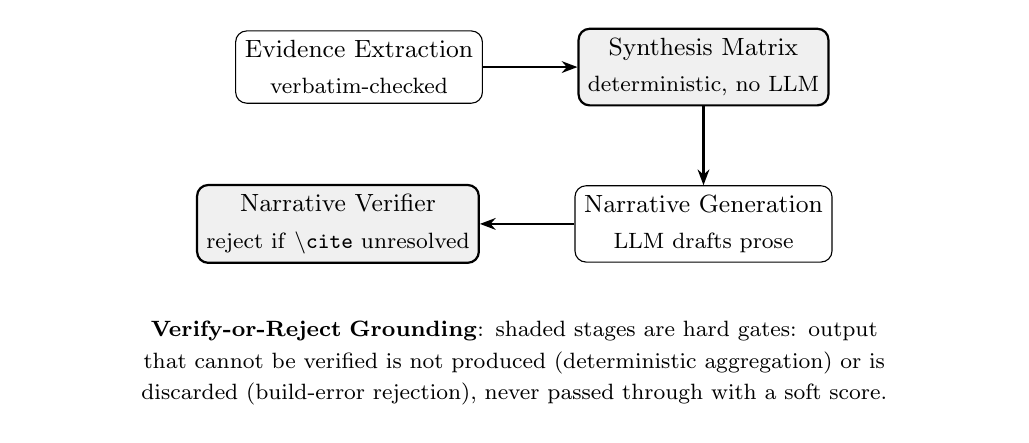
\begin{tikzpicture}[
 node distance=10mm and 12mm,
 box/.style={draw, rounded corners, minimum width=3.1cm, minimum height=9mm, align=center, font=\small},
 gate/.style={draw, rounded corners, minimum width=3.1cm, minimum height=9mm, align=center, font=\small, fill=gray!12, thick},
 arr/.style={-{Stealth[length=2mm]}, thick}
]
\node[box] (evi) {Evidence Extraction \\ \footnotesize verbatim-checked};
\node[gate, right=of evi] (mat) {Synthesis Matrix \\ \footnotesize deterministic, no LLM};
\node[box, below=of mat] (nar) {Narrative Generation \\ \footnotesize LLM drafts prose};
\node[gate, left=of nar] (ver) {Narrative Verifier \\ \footnotesize reject if \texttt{\textbackslash cite} unresolved};

\draw[arr] (evi) to (mat);
\draw[arr] (mat) to (nar);
\draw[arr] (nar) to (ver);

\node[fit=(ver)(nar), inner sep=0pt] (bottomrow) {};
\node[below=6mm of bottomrow, font=\footnotesize, align=center, text width=\linewidth]
 {\textbf{Verify-or-Reject Grounding}: shaded stages are hard gates: output that cannot be verified is not produced (deterministic aggregation) or is discarded (build-error rejection), never passed through with a soft score.};
\end{tikzpicture}
\caption{The evidence-grounded synthesis sub-pipeline. Shaded boxes are verify-or-reject gates; unshaded boxes are ordinary LLM-driven generation stages that feed into a gate.}
\label{fig:architecture}
\end{figure}

\section{Proposed Method: Verify-or-Reject Grounding}
\label{sec:method}

We define a pipeline stage as \textbf{scored-grounded} if it emits output alongside a confidence signal (a score, flag, or review-queue entry) that a downstream consumer may act on or ignore, and as \textbf{verify-or-reject grounded} if the stage's output type itself excludes unverifiable content: either because the stage is deterministic over already-verified inputs (introducing no new hallucination surface), or because an explicit verification step discards non-conforming output before it can propagate. The distinction matters because scored grounding is a property of the \emph{output}, inspectable but skippable, whereas verify-or-reject grounding is a property of the \emph{pipeline itself}, which a downstream stage cannot bypass by ignoring a score field it was never given -- the same reject-by-default logic behind the fail-safe-defaults principle in classical protection-system design~\cite{saltzer1975protection}, applied here to citation grounding instead of access control.

Algorithm~\ref{alg:vorg} formalizes the narrative-verification instance of the pattern used in \S\ref{sec:architecture}. Rather than checking each sentence against the evidence table by linear scan, as a naive scored-grounding implementation would, \textsc{VoRG-Certify} first compiles the evidence table into a hash index, then certifies the entire narrative in a single pass, so that certification cost scales with the size of the narrative and evidence table separately rather than with their product.

\captionof{algorithm}{\textsc{VoRG-Certify}: Linear-Time Verify-or-Reject Narrative Certification}
\label{alg:vorg}
\begin{algorithmic}[1]
\Require Evidence table $E = \{e_1, \dots, e_n\}$, each row keyed by a unique citation key $\kappa(e_i)$; generated narrative $N = (s_1, \dots, s_m)$
\Ensure Certified narrative $N'$ containing only sentences whose citations resolve to $E$; rejection log $R$ recording every discarded sentence and its cause
\Function{BuildIndex}{$E$}
 \State $H \gets$ empty hash map
 \For{each $e_i \in E$}
 \State $H[\kappa(e_i)] \gets e_i$ \Comment{expected $O(1)$ insert}
 \EndFor
 \State \Return $H$
\EndFunction
\Statex
\Function{Certify}{$N$, $H$}
 \State $N' \gets \emptyset$;\ $R \gets \emptyset$
 \For{each sentence $s_j \in N$} \Comment{single pass, $j = 1, \dots, m$}
 \State $K_j \gets \Call{ExtractKeys}{s_j}$ \Comment{one regex scan, $O(|s_j|)$}
 \If{$K_j = \emptyset$}
 \State $R \gets R \cup \{(s_j, \textsc{NoClaim})\}$ \Comment{no grounding claim at all}
 \ElsIf{$\exists\, k \in K_j$ such that $k \notin H$}
 \State $R \gets R \cup \{(s_j, \textsc{Unresolved})\}$ \Comment{build error, $O(1)$ lookup per key}
 \Else
 \State $N' \gets N' \cup \{s_j\}$
 \EndIf
 \EndFor
 \State \Return $(N', R)$
\EndFunction
\end{algorithmic}

\paragraph{Complexity.} Let $n = |E|$, let $m$ be the number of generated sentences, and let $M = \sum_{j=1}^m |s_j|$ be the total length of the narrative. \Call{BuildIndex}{} performs $n$ hash insertions, $O(n)$ expected time and $O(n)$ space for the index. \Call{Certify}{} makes one linear pass over $N$: key extraction is a single regex scan per sentence, contributing $O(M)$ in total across all sentences, and each extracted key is resolved against $H$ in expected $O(1)$, contributing $O(m)$ for the lookups. The full algorithm therefore runs in
\[
T(n, M) = O(n + M) \qquad \text{expected time,} \qquad S(n, m) = O(n + m) \qquad \text{auxiliary space,}
\]
since $m \le M$ and the output $N'$ and log $R$ together hold at most $m$ sentence references. This is linear in the combined size of the evidence table and the narrative and has no dependence on $n \cdot m$. The linear-scan alternative — checking every sentence's citation against every evidence row, the implicit cost of a scored-grounding pipeline with no index structure — costs $O(n \cdot m)$; \textsc{VoRG-Certify}'s hash-indexed design removes this quadratic term, which matters because $n$ and $m$ both grow with corpus size, so certification remains linear rather than quadratic as the evidence base scales. The same index-then-certify structure applies to contradiction judgments (indexed by claim-pair key, discarded below the Likert threshold rather than reported with a low score) and journal-metadata fields (indexed by source, tagged \texttt{unknown} when absent rather than interpolated), so the $O(n+M)$ bound extends to those subsystems under the same argument. Table~\ref{tab:contrast} contrasts the approach with the scored-grounding baseline typified by Li et al.~\cite{li2025enhancing}.

\begin{table}[h]
\centering
\caption{Scored grounding vs. verify-or-reject grounding.}
\label{tab:contrast}
\begin{tabular}{@{}p{3.6cm}p{5.3cm}p{5.3cm}@{}}
\toprule
& \textbf{Scored grounding} & \textbf{Verify-or-reject grounding} \\
\midrule
Unverifiable output & Emitted with a low score/flag & Not emitted; build error raised \\
Downstream dependence & Consumer must check the score & Consumer receives only verified output \\
Aggregation steps & Often LLM-driven, itself a hallucination source & Deterministic where possible (no new LLM surface) \\
Failure visibility & Silent unless score is inspected & Explicit, logged rejection \\
\bottomrule
\end{tabular}
\end{table}

\section{Evaluation}
\label{sec:evaluation}

\subsection{Setup}

We evaluate on a single gold-annotated topic, \textit{graph neural networks in drug discovery}, using the system's own evaluation harness. The frozen corpus contains 10 papers retrieved from CrossRef; critically, only one of the ten carries a non-empty abstract in the CrossRef metadata (the remaining nine are title/DOI-only records), which we treat as a first-class limitation of this evaluation rather than obscure. Gold annotations were authored by the present authors by independently checking pipeline-extracted claims against the one paper with genuine abstract text (yielding three verbatim gold claims), and by independently judging genuine research-gap and contradiction labels against all ten paper titles and the corpus's own composition, rather than by rubber-stamping the pipeline's own output. We compare three configurations, each repeated three times (temperature 0.3, provider Groq \texttt{openai/gpt-oss-120b} where an LLM call is used):
\begin{itemize}
 \item \textbf{Full pipeline (LLM mode):} all LLM-backed stages active.
 \item \textbf{Pattern-mode ablation:} LLM-backed extraction stages replaced by regex/rule-based fallbacks, isolating how much of the pipeline's performance depends on the LLM calls themselves.
 \item \textbf{Naive baseline:} a single prompt containing all ten frozen abstracts/titles, asked in one shot for claims, contradictions, and gaps, scored with the identical matcher.
\end{itemize}
This baseline isolates the effect of decomposing extraction into per-paper, per-claim stages; it is not a matched scored-grounding ablation (an implementation that emits the same per-claim output alongside a confidence score instead of enforcing rejection), so the comparisons below should be read as evidence that structured decomposition helps, not as a direct test of verify-or-reject grounding against scored grounding on identical output. \S\ref{sec:limitations} returns to this scoping.

\subsection{Results}

\begin{table}[h]
\centering
\caption{Claim-extraction performance, mean $\pm$ SD over 3 runs, against 3 gold-annotated claims.}
\label{tab:claims}
\begin{tabular}{@{}lccc@{}}
\toprule
Configuration & Precision & Recall & F1 \\
\midrule
Full pipeline (LLM mode) & 0.294 $\pm$ 0.042 & 0.889 $\pm$ 0.192 & 0.442 $\pm$ 0.070 \\
Pattern-mode ablation & 0.439 $\pm$ 0.211 & 0.667 $\pm$ 0.000 & 0.510 $\pm$ 0.152 \\
Naive single-LLM baseline & 0.104 $\pm$ 0.006 & 0.333 $\pm$ 0.000 & 0.158 $\pm$ 0.007 \\
\bottomrule
\end{tabular}
\end{table}

Both the full pipeline and the pattern-mode ablation substantially outperform the naive single-prompt baseline (F1 2.8$\times$ and 3.2$\times$ higher, respectively), indicating that decomposing extraction into per-paper, per-claim stages helps regardless of whether an LLM or a rule-based extractor performs each stage. The pattern-mode ablation's point estimate is competitive with, and in this small sample nominally higher than, the full LLM pipeline; this is attributed largely to the gold set's small size (three claims, all near-verbatim sentences from the one paper with real abstract text), which mechanically favours a regex extractor tuned to sentence boundaries. This result is reported as such rather than as evidence that rule-based extraction generally outperforms LLM extraction: precision variance for pattern mode ($\pm$0.211) is far higher than for the full pipeline ($\pm$0.042), consistent with a rule-based extractor whose hit rate depends heavily on incidental sentence structure.

\textbf{Contradiction detection.} Across all nine runs (three configurations $\times$ three repeats), the false-positive rate on the two hand-labelled negative pairs was 0.0; the system never asserted a contradiction between the two pairs independently verified as compatible. No gold-positive contradictions exist in this small corpus (the eight extracted claims are non-overlapping scoping statements rather than conflicting empirical results), so recall is undefined; this is a precision-only sanity check, not a full validation of the contradiction judge.

\textbf{Research-gap detection.} Gap recall against two independently authored gold gaps was 0.0 in two of three full-pipeline runs and 0.5 in the third (mean 0.17); precision@3 was 0.0 in every run. This is a genuine negative result. Inspecting the raw predictions surfaces a concrete failure mode: one run's top-ranked gap claimed \emph{``no studies have applied graph-based generative models ... for de novo molecular generation''}, directly contradicted by the reviewed corpus's own sixth paper, \emph{``Molecular generative Graph Neural Networks for Drug Discovery''} (a corpus item, not itself a formal literature citation of this paper). The gap-detection stage is, notably, the one component of the pipeline described in \S\ref{sec:architecture} that does \emph{not} yet apply verify-or-reject grounding: a candidate gap is generated and ranked, but never checked against the titles or content of the very corpus it is judging. This failure is informative beyond the bare recall number: it identifies precisely which architectural gap in the reference system produced the empirical weakness, and it directly motivates extending Algorithm~\ref{alg:vorg}'s pattern (reject a claim that contradicts available evidence) to gap description as future work.

\subsection{Cost}

Mean cost per full-pipeline run was \$0.008 $\pm$ \$0.002 (16.3 $\pm$ 1.5 LLM calls), against \$0.002 $\pm$ \$0.001 for the pattern-mode ablation and \$0.001 (constant, 1 call) for the naive baseline. Parse failures (malformed LLM JSON discarded rather than guessed at) occurred in one of nine total runs across all configurations, after a schema-validation defect was identified and fixed during this evaluation (see \S\ref{sec:limitations}).

\section{Discussion}
\label{sec:discussion}

The two gated stages and the one ungated stage diverge in exactly the way the architecture predicts. Claim extraction and contradiction detection each pass every candidate output through an explicit accept/reject check before it can be reported, and both come out ahead of the ungated naive baseline (Table~\ref{tab:claims}) with a 0.0 false-positive rate on the hand-labelled contradiction pairs. Research-gap detection has no equivalent check -- a candidate gap is generated and ranked but never compared against the very corpus it is judging -- and it is precisely there that the pipeline produced a false claim contradicted by a paper already in the reviewed corpus. This result was not introduced as a separate test to demonstrate the value of VoRG; it emerged during evaluation of the existing pipeline, and the location of the failure lines up with the one architectural gap identified in \S\ref{sec:architecture}.

The journal-metadata reconciliation component illustrates the same discipline applied to structured rather than narrative output: values are classified as verified, estimated, or unknown, and differences between sources are surfaced in a discrepancy field rather than silently averaged. Nothing about the underlying idea is specific to literature review -- any pipeline that generates text or structured records from retrieved sources can apply the same accept/reject check before passing output downstream, in place of a confidence score a later stage might not act on.

The current results should not be taken as evidence that verify-or-reject grounding solves hallucination in every setting. The evaluation is small and limited to one topic, and the pattern-mode ablation performed better than the full LLM pipeline on claim-extraction F1. The main value of the evaluation is instead that it identifies where verification is already useful and where its absence leads to a concrete failure. Extending the same principle to research-gap detection and testing it on larger and more varied corpora are therefore the most direct next steps.

\section{Limitations}
\label{sec:limitations}

This evaluation has several limitations. First, it covers a single topic and a single set of human annotators rather than the multi-topic, multi-annotator gold standard that the evaluation harness is designed to support. Second, nine of the ten papers in the frozen corpus contain no abstract text in their CrossRef metadata, limiting the independently verifiable gold set to three sentences from a single paper; this is primarily a corpus-acquisition limitation, but it also limits the statistical power of the evaluation. Third, two pre-existing implementation defects were identified and fixed during the evaluation: a retired LLM model identifier that caused fallback to a degraded extraction mode, and a schema-validation issue that rejected valid null-valued fields from certain LLM providers. The reported results therefore reflect the corrected implementation rather than the system in its original state. Fourth, each configuration was evaluated over only three runs; this satisfies the minimum reproducibility requirement of the evaluation harness, but the resulting variance estimates should be considered indicative rather than precise. Fifth, the evaluation does not include a matched scored-grounding ablation: a pipeline variant that emits the same per-claim output alongside a confidence score or review flag instead of enforcing rejection. The naive baseline in \S\ref{sec:evaluation} tests whether decomposition into per-paper, per-claim stages helps, not whether rejection outperforms scoring on otherwise identical output; comparing verify-or-reject grounding directly against a scored-grounding ablation, with a fixed decomposition and only the accept/reject decision varied, is the most direct way to isolate the paper's central architectural claim and is left as the primary next experiment. Finally, several supporting citations include explicit quartile caveats because Q1 status could not be independently confirmed for every subtopic discussed. These limitations are reported to provide a clear account of the evaluation scope and evidence quality.

\section{Conclusion}

We presented Verify-or-Reject Grounding (VoRG) and implemented it across literature synthesis, contradiction detection, and journal-metadata reconciliation.

The evaluation shows that the full pipeline performs substantially better than the naive single-prompt baseline for claim extraction, although the pattern-mode ablation achieved a higher F1 score in this small evaluation. The results also exposed a clear limitation: research-gap detection, not protected by the same verification mechanism, produced low recall and a false positive contradicted by the reviewed corpus. This provides a concrete direction for extending the approach.

Future work will apply the verify-or-reject mechanism to research-gap detection, increase the size and diversity of the evaluation corpus, and use multiple annotators to produce a stronger gold standard. These extensions will help determine whether the observed benefits of VoRG remain consistent across different topics and datasets.

\section*{Data and Code Availability}

The reference implementation, evaluation harness, and gold-annotation files used in \S\ref{sec:evaluation} are available at \url{https://github.com/harishvidyarthcsecs/Research}.

\section*{Conflict of Interest}

The authors declare no conflict of interest.

\bibliographystyle{unsrt}
\bibliography{references}

\end{document}
